\documentclass{uofa-eng-assignment}
\usepackage{pythonhighlight}


\usepackage{float}
\usepackage{amsmath}
\usepackage{enumerate}% http://ctan.org/pkg/enumerate
\usepackage{lipsum, afterpage}
\usepackage{hyperref}
\usepackage{amsmath, amsthm, amssymb, amsfonts, physics}
\usepackage{mathtools}
\usepackage{graphicx}
\usepackage{fdsymbol}
\usepackage{xcolor}
\usepackage{piton}

\hypersetup{
    colorlinks=true,
    linkcolor=blue,
    filecolor=magenta,
    urlcolor=cyan,
    pdftitle={Overleaf Example},
    pdfpagemode=FullScreen,
}

\graphicspath{ {./images/} }

\DeclareRobustCommand{\rchi}{{\mathpalette\irchi\relax}}
\newcommand{\infdiv}{D\infdivx}
\newcommand{\irchi}[2]{\raisebox{\depth}{$#1\chi$}} % inner command, used by \rchi
\newcommand\aug{\fboxsep=-\fboxrule\!\!\!\fbox{\strut}\!\!\!}
\newcommand*{\name}{\textbf{Luke Nguyen}}
\newcommand*{\id}{\textbf{D5850A}}
\newcommand*{\course}{Statistical Methods and Data Analysis (EN.625.603)}
\newcommand*{\assignment}{Project 2}

\begin{document} \maketitle
%%%%%%%%%%%%%%%%%%%%%%%%%%%%%%%%%%%%%%%%%%%%%%%%%%%%%%%%%%%%%%%%%%%%%%%%%%%%%%%%%%%%%%%%%%%%%%%%%%%%    
\begin{enumerate}
    %%%%%%%%%%%%%%%%%%%%%%%%%%%%%%%%%%%%%%%%%%%%%%%%%%%%%%%%%%%%%%%%%%%%%%%%%%%%%%%%%%%%%%%%%%%%%%%%%%%%    
    %%%%%%%%%%%%%%%%%%%%%%%%%%%%%%%%%%%%%%%%%%%%%%%%%%%%%%%%%%%%%%%%%%%%%%%%%%%%%%%%%%%%%%%%%%%%%%%%%%%%    
    %%%%%%%%%%%%%%%%%%%%%%%%%%%%%%%%%%%%%%%%%%%%%%%%%%%%%%%%%%%%%%%%%%%%%%%%%%%%%%%%%%%%%%%%%%%%%%%%%%%%    
    %%%%%%%%%%%%%%%%%%%%%%%%%%%%%%%%%%%%%%%%%%%%%%%%%%%%%%%%%%%%%%%%%%%%%%%%%%%%%%%%%%%%%%%%%%%%%%%%%%%%    
    %%%%%%%%%%%%%%%%%%%%%%%%%%%%%%%%%%%%%%%%%%%%%%%%%%%%%%%%%%%%%%%%%%%%%%%%%%%%%%%%%%%%%%%%%%%%%%%%%%%%    
    \item[] \textbf{Question 1} \\
        Get to know your data. Make histograms and summary statistics of your data to get a sense of
        distributions.
        \begin{enumerate}
            \item What is the average value of birthweight for mothers who smoke? For mothers who
                  don’t smoke?
        \end{enumerate}
        \textbf{Solution}
        \begin{figure}[H]
            \centering
            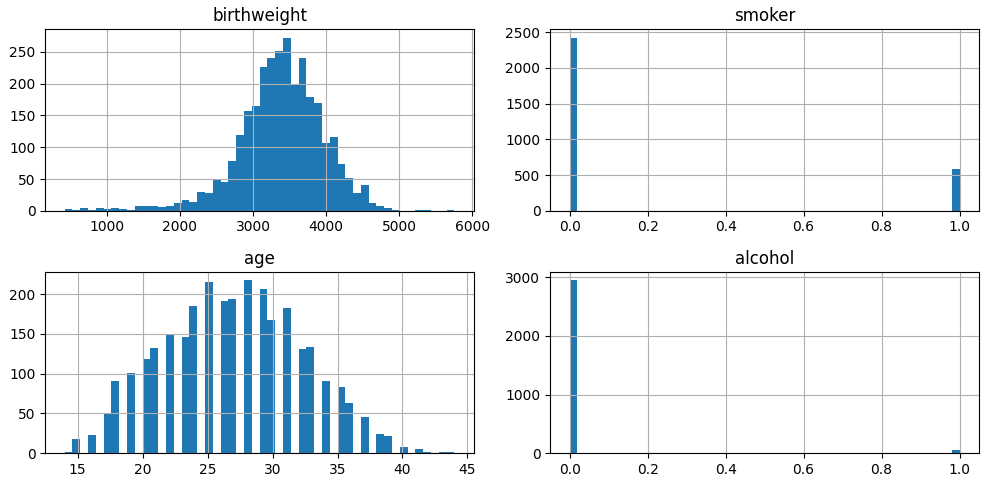
\includegraphics[width=0.558\textwidth]{p2-1-1.png}
        \end{figure}
        \begin{figure}[H]
            \centering
            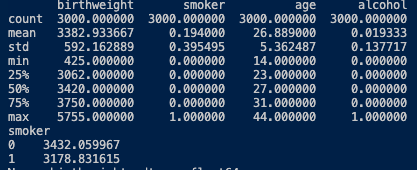
\includegraphics[width=0.55\textwidth]{p2-1-2.png}
        \end{figure}
        From Python and Pandas, we can see that the
        average value of birthweight
        for mothers who smoke is 3178.83 and for mothers who don't smoke is 3432.06. \\
    \item[] \textbf{Question 2} \\
        Consider associations. Plot each predictor (variables 2 through 11 in the pdf data description)
        against the response (birthweight). You could also do a quick line fit or get its correlation.
        Correlation is with “cor()”. A line fit can be achieved using the linear model function.
        Try for regressions 2 through 11.
        \begin{enumerate}
            \item What does a regression of birthweight on the binary variable smoker suggest
                  about the relationship between maternal smoking and infant birthweight?
            \item Do you think the regression above accurately captures the impact of smoking on
                  birthweight? (Consider the assumptions of the linear regression model and
                  whether they are met. Hint: do you think smoking is uncorrelated with other
                  factors that cause low birthweight?)
            \item Regress birthweight on smoker, alcohol, and nprevist. Explain why the exclusion
                  of these variables could lead to a biased regression coefficient in (a) above.
                  Is the estimated effect of smoking on birthweight substantially different from
                  the regression in (a) above?
            \item Jane smoked during her pregnancy, did not drink alcohol, and had 8 prenatal
                  care visits. Use the regression in (c) to predict the birthweight of Jane’s
                  infant.
        \end{enumerate}
        \textbf{Solution} \\
        All plots and regression lines and fitting model for each predictor against birthweight are shown below.

        \begin{figure}[H]
            \centering
            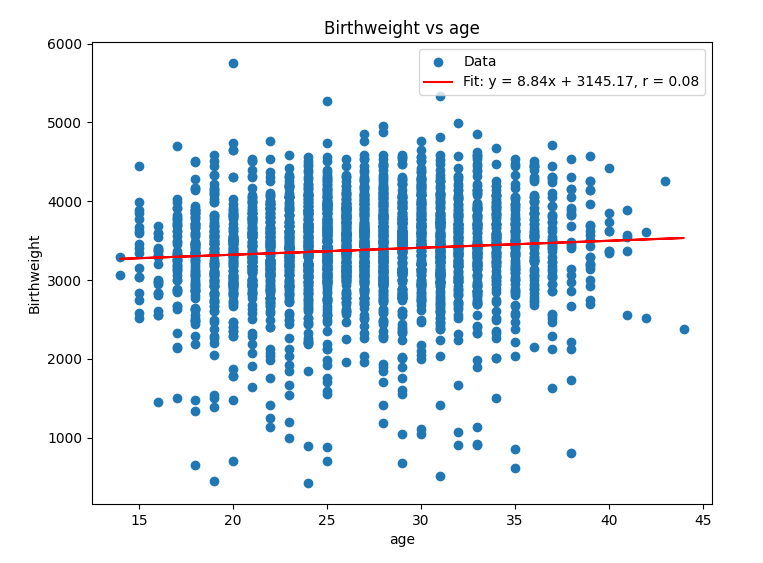
\includegraphics[width=0.55\textwidth]{bw-age.png}
        \end{figure}
        \begin{figure}[H]
            \centering
            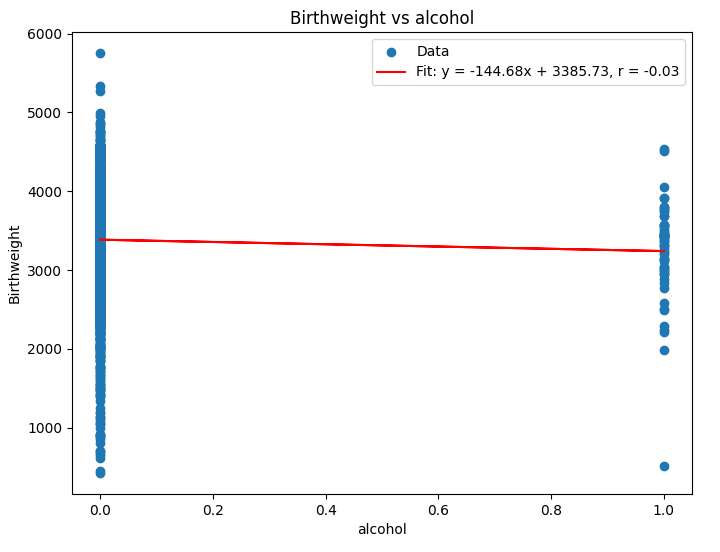
\includegraphics[width=0.55\textwidth]{bw-alco.png}
        \end{figure}
        \afterpage{%
            \clearpage % 
            \begin{figure}[H]
                \centering
                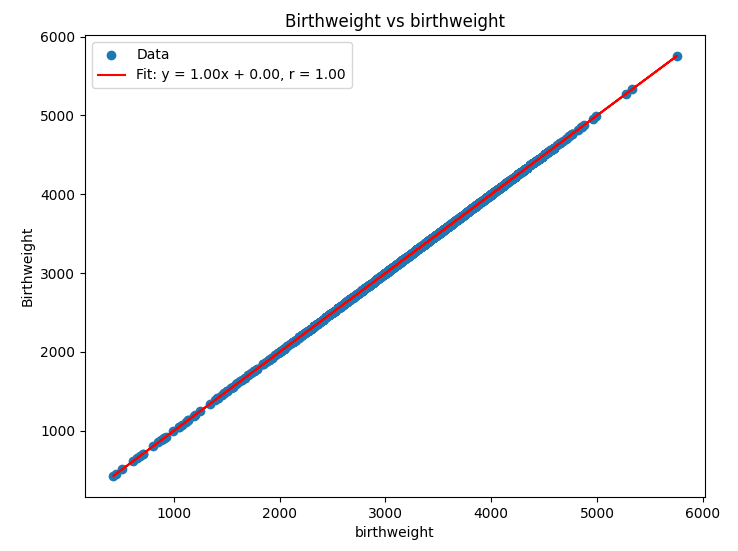
\includegraphics[width=0.55\textwidth]{bw-bw.png}
            \end{figure}
            \begin{figure}[H]
                \centering
                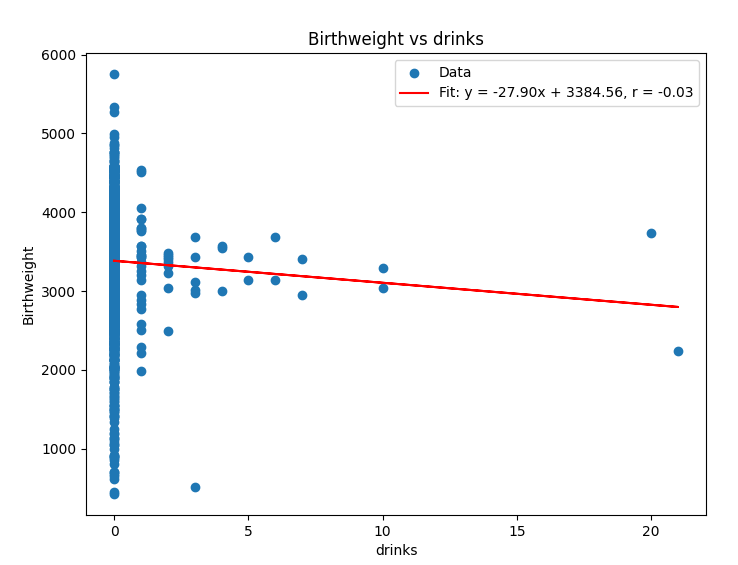
\includegraphics[width=0.55\textwidth]{bw-drink.png}
            \end{figure}
            \begin{figure}[H]
                \centering
                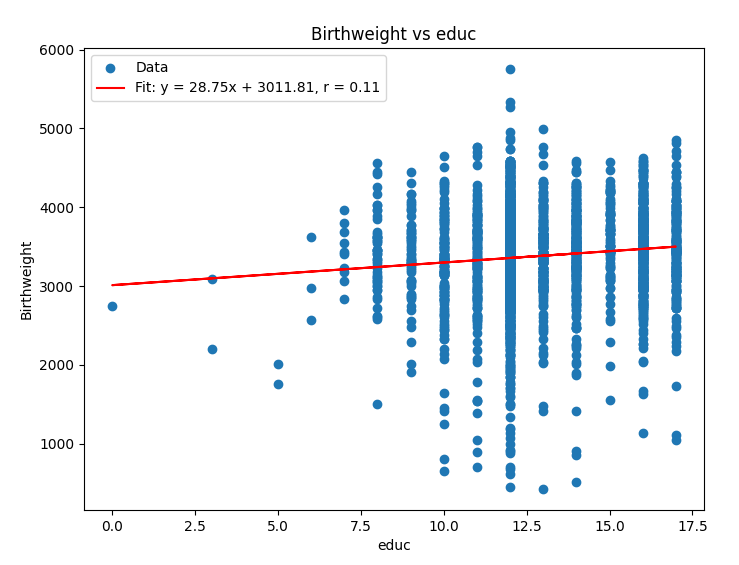
\includegraphics[width=0.55\textwidth]{bw-edc.png}
            \end{figure}
            \begin{figure}[H]
                \centering
                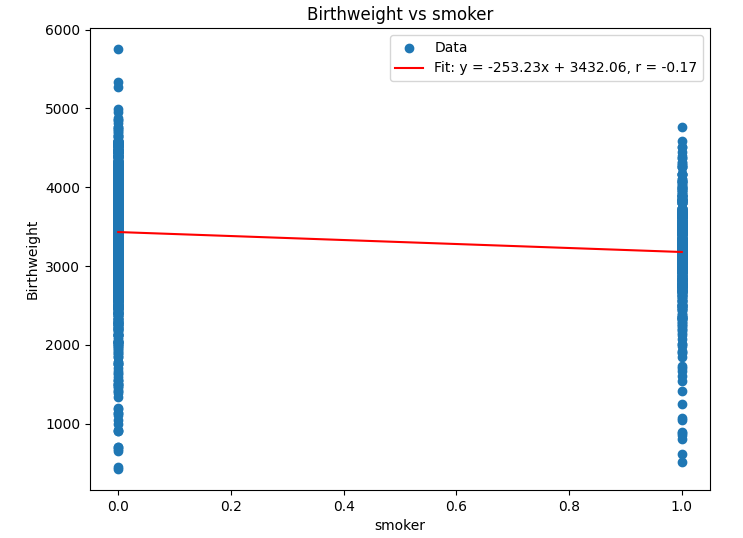
\includegraphics[width=0.55\textwidth]{bw-smo.png}
            \end{figure}
            \begin{figure}[H]
                \centering
                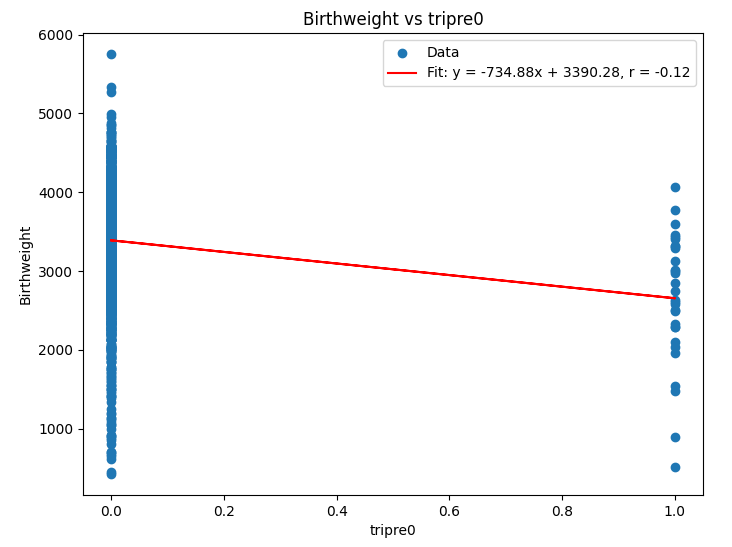
\includegraphics[width=0.55\textwidth]{bw-trip0.png}
            \end{figure}
            \begin{figure}[H]
                \centering
                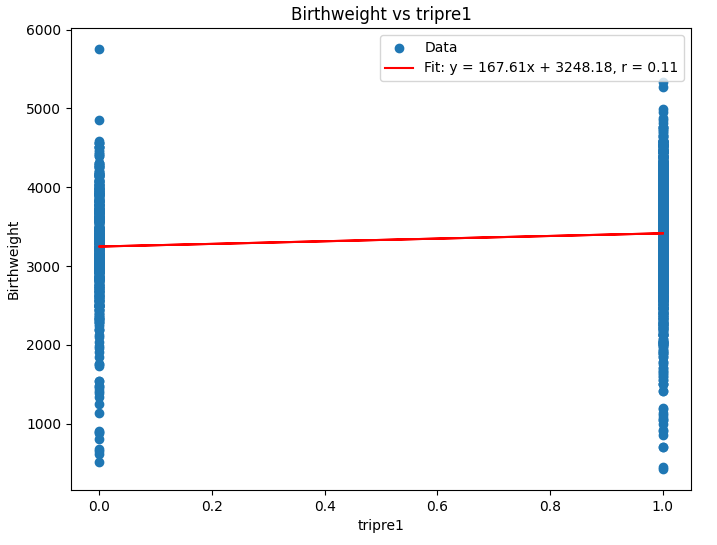
\includegraphics[width=0.55\textwidth]{bw-trip1.png}
            \end{figure}
            \begin{figure}[H]
                \centering
                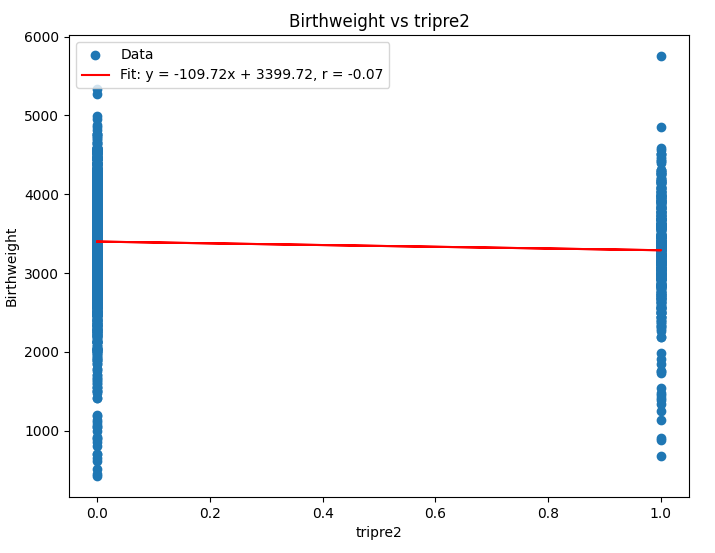
\includegraphics[width=0.55\textwidth]{bw-trip2.png}
            \end{figure}
            \begin{figure}[H]
                \centering
                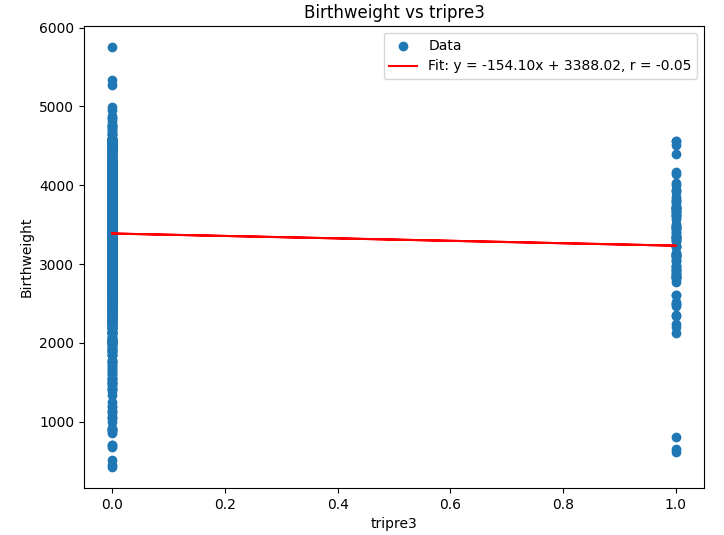
\includegraphics[width=0.55\textwidth]{bw-trip3.png}
            \end{figure}
            \begin{figure}[H]
                \centering
                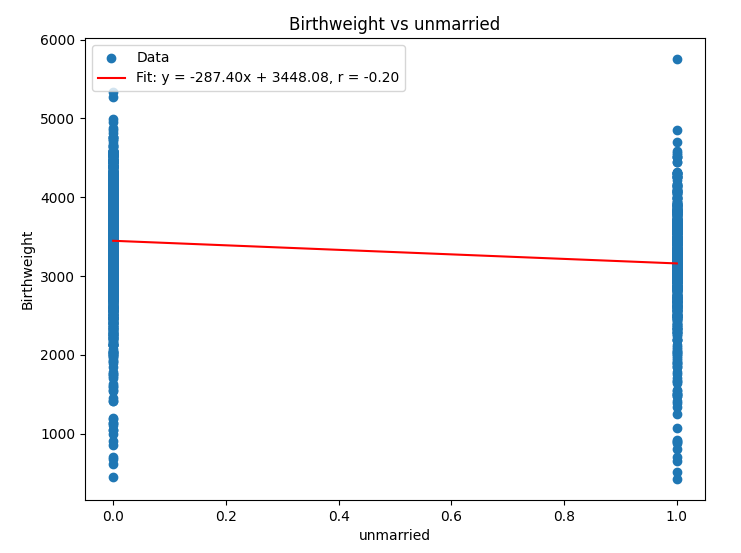
\includegraphics[width=0.55\textwidth]{bw-uma.png}
            \end{figure}
        }\clearpage
        \begin{enumerate}
            \item The fitting model for the regression of birthweight on the binary variable
                  smoker is
                  \begin{equation*}
                      \text{birthweight} = 3369.58 - 254.47 \times \text{smoker}
                  \end{equation*}
                  The regression suggests that the birthweight of infants whose mothers smoke is
                  254.47 grams less than the birthweight of infants whose mothers don't smoke.
            \item It might not be accurate because the assumptions of the linear regression model
                  might not be met. For example, smoking might be correlated with other factors
                  that cause low birthweight, one example is age of mother. The younger the
                  mother is, the more likely she is to smoke and the more likely her infant is to
                  have low birthweight. Plot and regression line and fitting model of age of
                  mother against birthweight are shown below \\
                  \begin{figure}[H]
                      \centering
                      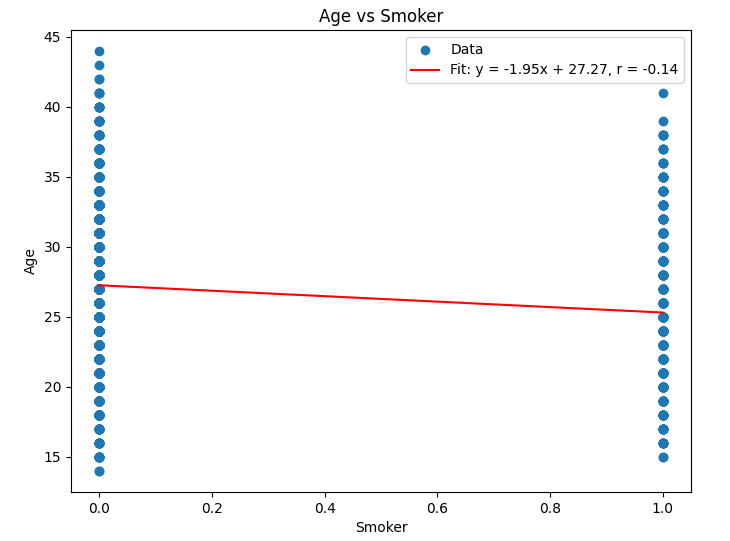
\includegraphics[width=0.55\textwidth]{smo-age.png}
                  \end{figure}
            \item Regressing birthweight on smoker, alcohol, and nprevist, we have
                  \begin{equation*}
                      \text{birthweight} = 3051.2486 - 217.5801 \times \text{smoker} - 30.4913 \times \text{alcohol} + 34.0699 \times \text{nprevist}
                  \end{equation*}
                  The exclusion of these variables could lead to a biased regression coefficient
                  in (a) above because
                  \begin{enumerate}
                      \item The estimated effect of smoking on birthweight is -254.47 grams if regress
                            birthweight against smoker only
                      \item The estimated effect of smoking on birthweight is -217.58 grams if regress
                            birthweight against smoker, alcohol, and nprevist
                  \end{enumerate}
                  And the estimated effect of smoking on birthweight is substantially different.
                  \begin{figure}[H]
                      \centering
                      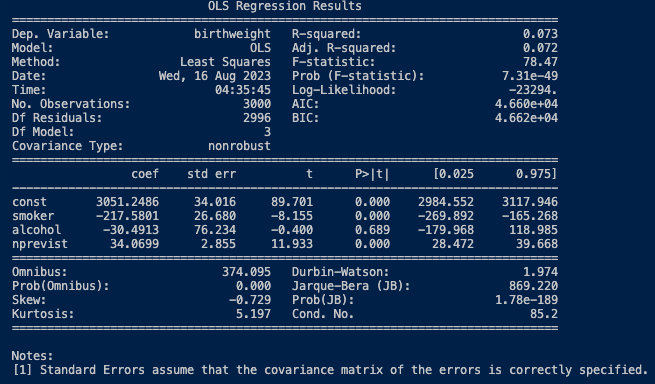
\includegraphics[width=0.65\textwidth]{p2-2-c.png}
                  \end{figure}
            \item Jane smoked, did not drink alcohol and had 8 prenatal care visits. Her infant's
                  birthweight is
                  \begin{align*}
                      \text{birthweight} & = 3051.2486 - 217.5801 \times 1 - 30.4913 \times 0 + 34.0699 \times 8 \\
                                         & = 3106.2277
                  \end{align*}
        \end{enumerate}
    \item[] \textbf{Question 3} \\
        An alternative way to control for prenatal visits is to use binary variables tripre0 through
        tripre3. Regress birthweight on smoker, alcohol, tripre0, tripre2, and tripre3.
        \begin{enumerate}
            \item Why is tripre1 excluded from the model? What happens if you include it in the
                  regression?
            \item The estimated coefficient on tripre0 is large and negative. What does this
                  coefficient measure? Interpret its value.
            \item Interpret the value of the estimated coefficients on tripre2 and tripre3.
            \item Does the regression in (3) explain a larger fraction of the variance in
                  birthweight than the regression in (2c)? (Hint: consider $R^2$.)
        \end{enumerate}
        \textbf{Solution} \\
        The fitting model for the regression of birthweight on smoker, alcohol, tripre0, tripre2, is as follows
        \begin{figure}[H]
            \centering
            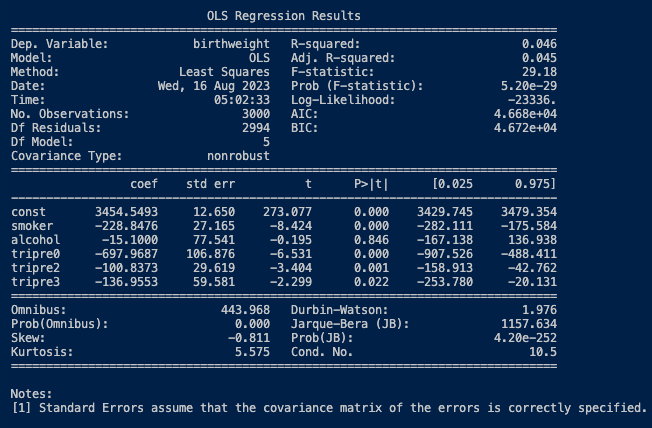
\includegraphics[width=0.70\textwidth]{p2-3.png}
        \end{figure}
        \begin{enumerate}
            \item tripre1 is excluded from the model because it is a linear combination of
                  tripre0, tripre2, and tripre3. If we include it in the regression, the
                  regression would be perfect multicollinearity overparameterized on tripre0,
                  tripre1, tripre2, and tripre3.
                  \begin{figure}[H]
                      \centering
                      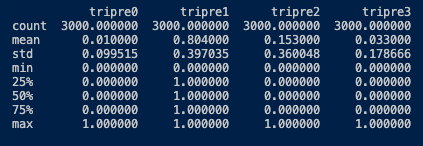
\includegraphics[width=0.55\textwidth]{p2-3-a.png}
                  \end{figure}
                  As showing in the figure above
                  \begin{align*}
                      \overline{tripre1} = 1 - \overline{tripre0} - \overline{tripre2} - \overline{tripre3}
                  \end{align*}
            \item The estimated coefficient on tripre0 is large and negative. This coefficient
                  measures the difference in birthweight between infants whose mothers had no
                  prenatal visits and infants whose mothers had one or more prenatal visit. The
                  difference is 698 grams which is very substantial. This suggests that prenatal
                  visits has strong positive linear relationship with infant's birthweight. \\ By
                  common sense, having no prenatal visits could mean that the pregnant mother is
                  not aware of the importance of prenatal visits, or she is not able to afford,
                  both of which could be strong signs of not having enough resources to support
                  the infant's growth.
            \item The estimated coefficients on tripre2, tripre3 are -100.84 and -136.96
                  respectively. These coefficients measure the difference in birthweight between
                  infants whose mothers had first prenatal visit in the second/third trimester
                  and infants whose mothers had first prenatal visit in the first trimester or
                  none. It suggests that the earlier the mother has her first prenatal visit, the
                  more likely her infant is to have higher birthweight.
            \item $R^2$ in (2c) is 0.073, while $R^2$ in (3) is 0.046. The regression in (2c)
                  explains a larger fraction of the variance in birthweight than the regression
                  in (3).
        \end{enumerate}
    \item[] \textbf{Question 4} \\
        Consider adding an additional regressor: Regress birthweight on smoker, alcohol, nprevist, and
        unmarried.
        \begin{enumerate}
            \item Compare the coefficient on smoker in this regression to the coefficients on
                  smoker in regressions (2a) and (2c). What is the estimated effect of smoking on
                  birthweight in each regression?
            \item Interpret differences in estimated effects.
            \item Interpret the estimated effect of marital status on birthweight. Is the
                  coefficient on unmarried statistically significant? Is the magnitude of the
                  coefficient large?
            \item A family advocacy group notes that the large coefficient suggests that public
                  policies that encourage marriage will lead, on average, to healthier babies. Do
                  you agree? (Hint: consider some of the various factors that unmarried may be
                  controlling for and how this affects the interpretation of this coefficient).
        \end{enumerate} \newpage
        \textbf{Solution} \\
        The fitting model for the regression of birthweight on smoker, alcohol, nprevist, and unmarried is as follows
        \begin{figure}[H]
            \centering
            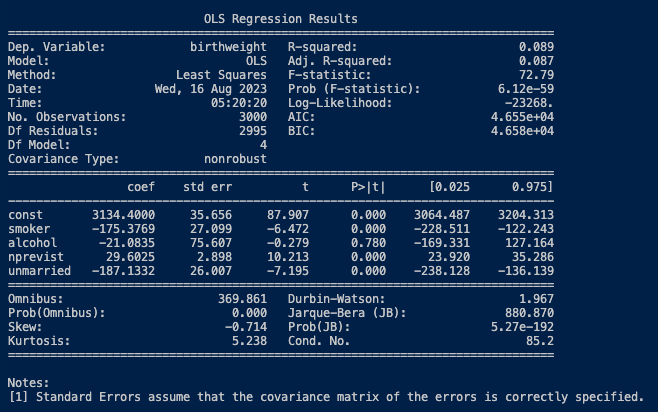
\includegraphics[width=0.70\textwidth]{p2-4.png}
        \end{figure}
        \begin{enumerate}
            \item Smoker coefficient in this regression is -175.38, while smoker coefficient in
                  (2a) is -254.47 and smoker coefficient in (2c) is -217.58. The estimated effect
                  \begin{enumerate}
                      \item In (2a) is lowering birthweight by 254.47 grams
                      \item In (2c) is lowering birthweight by 217.58 grams
                      \item In this regression is lowering birthweight by 175.38 grams
                  \end{enumerate}
            \item Smoker coefficient in this regression is less significant than smoker
                  coefficient in (2a) and (2c). This suggests that the estimated effect of
                  smoking on birthweight is less significant in this regression than in (2a) and
                  (2c), this is because the effect of smoking on birthweight is confounded by
                  unmarried in this regression. A possible explanation is that unmarried mothers
                  are more likely to smoke than married mothers, and unmarried mothers are more
                  likely to have lower birthweight infants than married mothers. Therefore, the
                  estimated effect of smoking on birthweight is less significant in this
                  regression than in (2a) and (2c).
            \item The coefficient on unmarried is statistically significant because $p$-value is
                  less than 0.05. The magnitude of the coefficient is -187 which is very large
                  because it would put the infant's birthweight at 0.31 standard deviations below
                  the mean, if the birthweight is normally distributed.
            \item Although the coefficient of unmarried is large and its effects on lowering
                  birthweight is statistically significant. We can't conclude that public
                  policies that encourage marriage will lead, on average, to healthier babies.
                  Because, unmarried could have strong positive linear relationship with other
                  regressors, such as smoking, alcohol, and nprevist which are all negatively
                  correlated with birthweight.
        \end{enumerate} \newpage
    \item[] \textbf{Question 5} \\
        Consider the other coefficients in this data set. Which do you think should be included in the
        regression?
        \begin{enumerate}
            \item Try adding in some of these additional variables. Share your findings and
                  conclusions.
            \item The data set includes babies born in Pennsylvania in 1989. Discuss the external
                  validity of your analysis for: (i) California in 1989, (ii) Illinois in 2015,
                  (iii) South Korea in 2014.
            \item Overall, explain your conclusions on how maternal smoking impacts birthweight
                  (hint: the regressions you’re running should be helping you see that isolating
                  the causal effect of smoking on birthweight is difficult because there are a
                  lot of other confounding variables).
        \end{enumerate}
        \textbf{Solution} \\
        Considering that age and education were not considered in the previous regressions, I am adding them in a new regression. \\
        The fitting model for the regression of birthweight on age and education is as follows
        \begin{figure}[H]
            \centering
            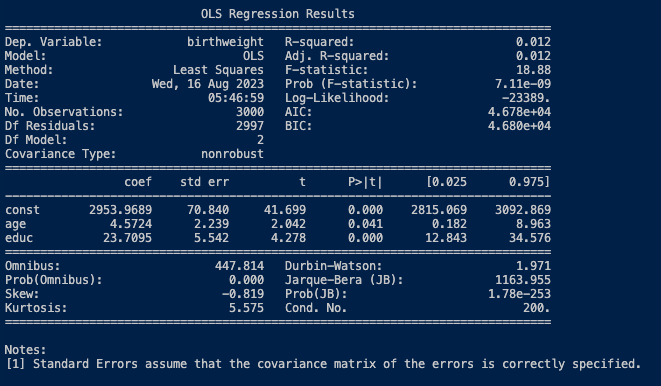
\includegraphics[width=0.70\textwidth]{p2-5.png}
        \end{figure}
        \begin{enumerate}
            \item The $p$-value of age is 0.041 which indicates that age has statistically
                  significant effect on birthweight. For each year older the mother is, the
                  infant's birthweight increases by 4.58 grams \\ The $p$-value of education is
                  0.000 which indicates that education has statistically significant effect on
                  birthweight. For each year of education the mother has, the infant's
                  birthweight increases by 23.71 \item
                  \begin{enumerate}
                      \item  Applying the analysis of this dataset Pennsylvania in 1989 to California in
                            1989 could be valid because the data is collected from the same year and the
                            same country. Thus, the culture and the environment are similar, and the effect
                            of unmarried, smoker, alcohol, and nprevist on birthweight should be similar.
                      \item Applying the analysis of this dataset Pennsylvania in 1989 to Illinois in 2015
                            will not be valid because the data is collected by two points in time and the
                            difference is almost 30 years. Thus, the culture and the environment have
                            changed a lot.
                      \item Applying the analysis of this dataset Pennsylvania in 1989 to South Korea in
                            2014 will be absolutely invalid, the culture and the environment are totally
                            different. Smoker, alcohol, age could even have positive linear relationship
                            with birthweight in South Korea.
                  \end{enumerate}
            \item Maternal smoking has negative linear relationship with birthweight. However,
                  isolating the causal effect of smoking on birthweight is difficult because
                  there are a lot of other confounding variables. For example, unmarried,
                  alcohol, age, and education are all confounding variables. The estimated effect
                  of smoking on birthweight is less significant in the regression of birthweight
                  on smoker, alcohol, nprevist, and unmarried than in the regression of
                  birthweight on smoker, alcohol, and nprevist. This is because unmarried is
                  confounding the effect of smoking on birthweight. A possible explanation is
                  that unmarried mothers are more likely to smoke than married mothers, and
                  unmarried mothers are more likely to have lower birthweight infants than
                  married mothers. Therefore, the estimated effect of smoking on birthweight is
                  less significant in the regression of birthweight on smoker, alcohol, nprevist,
                  and unmarried than in the regression of birthweight on smoker, alcohol, and
                  nprevist.
        \end{enumerate}
\end{enumerate}

\begin{python}
# All code used to generate the answers are below
    import pandas as pd
    import numpy as np
    import statsmodels.api as sm
    from scipy import stats
    import scipy.stats
    import matplotlib.pyplot as plt
    import pandas as pd
    import matplotlib.pyplot as plt
    import numpy as np
    from scipy.stats import linregress
    
    
    class WeightSmokingDataframe:
        df = None
        def __init__(self):
            file_path = 'weight_smoking.xlsx'
            file_sheet_name = 'Data'
            self.df = pd.read_excel(file_path, sheet_name=file_sheet_name)
    
    
    def part_1_solution():
        weightSmoking = WeightSmokingDataframe()
        print(weightSmoking.df[['birthweight', 'smoker', 'age', 'alcohol']].describe(
            include='all'))
        weightSmoking.df[['birthweight', 'smoker', 'age', 'alcohol']].hist(
            bins=50, figsize=(10, 5))
        average_birthweights = weightSmoking.df.groupby('smoker')[
            'birthweight'].mean()
        print(average_birthweights)
    
        plt.tight_layout()
        plt.show()
    
    
    def part_2_solution():
        weightSmoking = WeightSmokingDataframe()
        predictor_columns = weightSmoking.df.columns[1:12]
    
        for column in predictor_columns:
            slope, intercept, r_value, p_value, std_err = linregress(
                weightSmoking.df[column], weightSmoking.df['birthweight'])
            line = slope * weightSmoking.df[column] + intercept
            plt.figure(figsize=(8, 6))
            plt.scatter(weightSmoking.df[column],
                        weightSmoking.df['birthweight'], label='Data')
            plt.plot(weightSmoking.df[column], line, color='red',
                     label='Fit: y = {:.2f}x + {:.2f}, r = {:.2f}'.format(slope, intercept, r_value))
            plt.xlabel(column)
            plt.ylabel('Birthweight')
            plt.title('Birthweight vs ' + column)
            plt.legend()
            plt.show()
    
    
    def scatter_plot(x_col, y_col):
        df = WeightSmokingDataframe().df
        slope, intercept, r_value, p_value, std_err = linregress(
            df[x_col], df[y_col])
        line = slope * df[x_col] + intercept
        plt.figure(figsize=(8, 6))
        plt.scatter(df[x_col], df[y_col], label='Data')
        plt.plot(df[x_col], line, color='red',
                 label='Fit: y = {:.2f}x + {:.2f}, r = {:.2f}'.format(slope, intercept, r_value))
        plt.xlabel(x_col)
        plt.ylabel(y_col)
        plt.title(f'{y_col} vs {x_col}')
        plt.legend()
        plt.show()
    
    
    def part_2_solution_abcde():
        scatter_plot("smoker", "birthweight")
        scatter_plot("alcohol", "birthweight")
        scatter_plot("nprevist", "birthweight")
    
    
    def part_2_solution_c():
        df = WeightSmokingDataframe().df
        df = sm.add_constant(df)
        model_c = sm.OLS(df['birthweight'],
                         df[['const', 'smoker', 'alcohol', 'nprevist']])
        results_c = model_c.fit()
        print(results_c.summary())
    
    
    def part_3_solution():
        df = WeightSmokingDataframe().df
        df = sm.add_constant(df)
        model_c = sm.OLS(df['birthweight'],
                         df[['const', 'smoker', 'alcohol', 'tripre0', 'tripre2', 'tripre3']])
        results_c = model_c.fit()
        print()
        print(results_c.summary())
    
    
    def part_3a_solution():
        weightSmoking = WeightSmokingDataframe()
        print()
        print(weightSmoking.df[['tripre0', 'tripre1', 'tripre2', 'tripre3']].describe(
            include='all'))
    
    
    def part_4_solution():
        df = WeightSmokingDataframe().df
        df = sm.add_constant(df)
        model_c = sm.OLS(df['birthweight'],
                         df[['const', 'smoker', 'alcohol', 'nprevist', 'unmarried']])
        results_c = model_c.fit()
        print()
        print(results_c.summary())
    
    
    def part_5_solution():
        df = WeightSmokingDataframe().df
        df = sm.add_constant(df)
                         df[['const', 'age', 'educ']])
        results_c = model_c.fit()
        print()
        print(results_c.summary())
    
    
    if __name__ == '__main__':
        part_5_solution()
    
    \end{python}
%%%%%%%%%%%%%%%%%%%%%%%%%%%%%%%%%%%%%%%%%%%%%%%%%%%%%%%%%%%%%%%%%%%%%%%%%%%%%%%%%%%%%%%%%%%%%%%%%%%%    
\end{document}